
\documentclass[]{article}

%opening
\title{Node OS}
\author{Lennart Bittel, QuTech}
\usepackage{xcolor}
\usepackage{listings}
\usepackage{tikz}
\usetikzlibrary{positioning,fit,calc}
\usetikzlibrary{chains}
\usepackage{smartdiagram}
\usepackage{metalogo}
%\usepackage{dtklogos}

\definecolor{mGreen}{rgb}{0,0.6,0}
\definecolor{mGray}{rgb}{0.5,0.5,0.5}
\definecolor{mPurple}{rgb}{0.58,0,0.82}
\definecolor{backgroundColour}{rgb}{0.95,0.95,0.92}

\lstdefinestyle{CStyle}{
	backgroundcolor=\color{backgroundColour},   
	commentstyle=\color{mGreen},
	keywordstyle=\color{magenta},
	numberstyle=\tiny\color{mGray},
	stringstyle=\color{mPurple},
	basicstyle=\footnotesize,
	breakatwhitespace=false,         
	breaklines=true,                 
	captionpos=b,                    
	keepspaces=true,                 
	numbers=left,                    
	numbersep=5pt,                  
	showspaces=false,                
	showstringspaces=false,
	showtabs=false,                  
	tabsize=2,
	language=C
}
\begin{document}	
	\maketitle
\begin{figure}[h]
	\centering
\smartdiagram[bubble diagram]{Node OS,
		Scheduler, Network Stack, User Interface, Real-time\\ execution}
\end{figure}
\section{Overall outline}
Quantum Computers, especially in a network situation need new software specific to their properties. This involves new Internet protocols which are able to distribute entanglement efficiently using both features of repeater and distillation protocols.
Additionally, as long as qubits are not error corrected, decoherence will also demand real time operations.
\section{Scheduler}
The scheduler should give the following features:
\begin{itemize}
	\item Achieve optimal use of generated entanglement.
	\item Run multiple programs at the same time. This means that the program is able to 
\end{itemize}

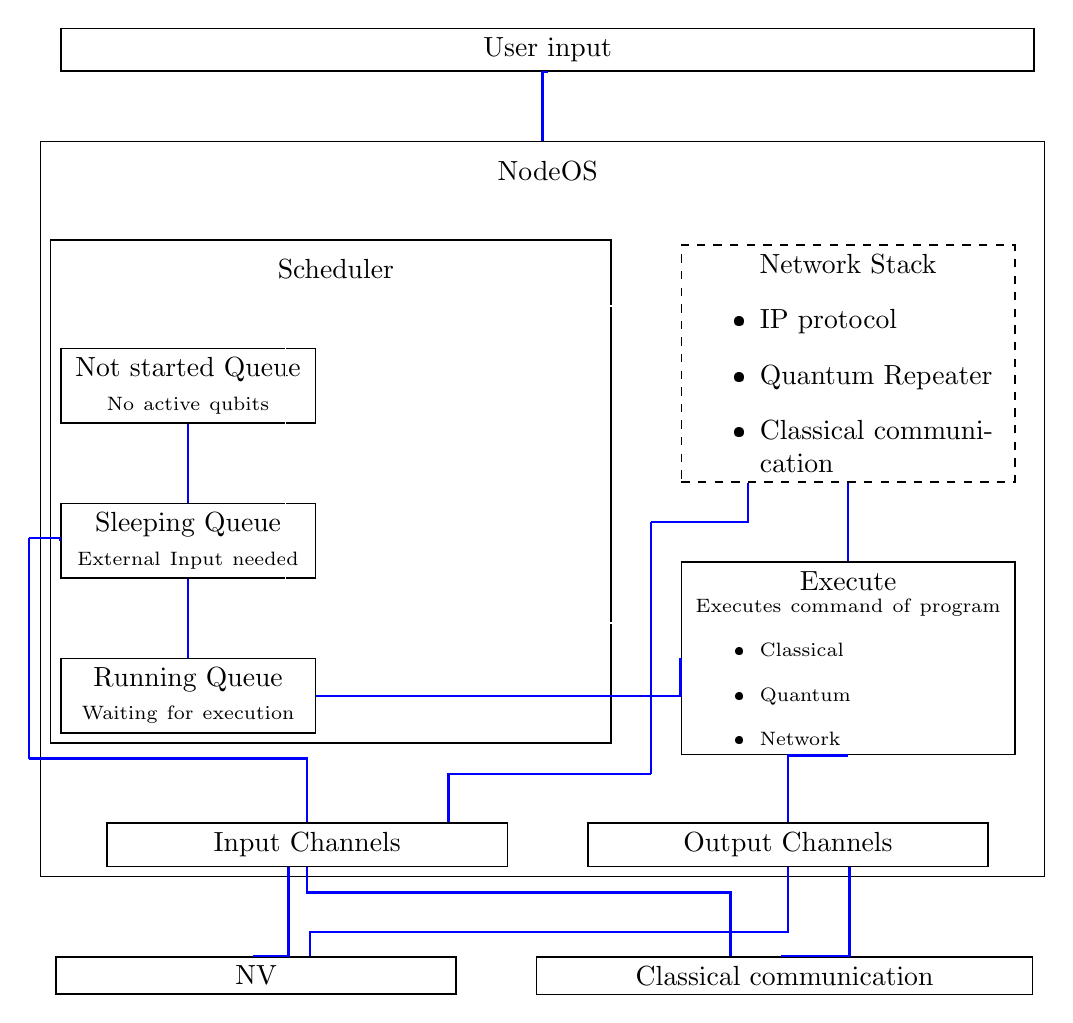
\begin{tikzpicture}[
every node/.style = {shape=rectangle,
	draw=black, semithick,
	text width=\linewidth,
	align=center,
	anchor=west
	}
]
\node (usr) {User input};
\node [below=of usr,draw=white] (NOS) {NodeOS};
\node[text width=6.5cm,below=of NOS.west,xshift=3.5cm,draw=white](Sch)
	{Scheduler};
	\node[text width=3cm,below=of Sch.west,xshift=1.5cm](NS){
			Not started Queue\\
			\scriptsize No active qubits
		};
	\node[text width=3cm,below=of NS](SL){
			Sleeping Queue\\
			\scriptsize External Input needed
		};
	\node[text width=3cm,below=of SL](RU){
			Running Queue\\
			\scriptsize Waiting for execution
		};
	\node (Scheduler)[draw=black, fit={(Sch) (SL) (NS) (RU)}] {};
\node[right=of NS,text width=4cm,xshift=-1.4cm,color=black!0,yshift=-1cm](Schd){
	\begin{itemize}
	\item Selects what task will run.
	\item Minimize execution time for important jobs.
	\item Minimize decoherence.
	\end{itemize}
	};	

\node[dashed,text width=4cm,right=of Sch,yshift=-1.2cm](NET){
		Network Stack
		\begin{itemize}
		\item IP protocol
		\item Quantum Repeater
		\item Classical communication
		\end{itemize}};
	\\
\node[below=of Scheduler,xshift=-0.3cm,text width=0.4\linewidth](In){
		Input Channels};
	\node[right=of In,xshift=0cm,text width=0.4\linewidth](Out){
		Output Channels};
	\node[below=of NET,text width=4cm] (EXE){
		Execute\\
		\scriptsize Executes command of program
		\begin{itemize}
			\item Classical
			\item Quantum
			\item Network
		\end{itemize}
	};
\node [draw=black, fit={(NOS) (Out) (Scheduler) (NET) }] (NODEOS){};
\node[below=of NODEOS,text width=0.4*\linewidth,xshift=-0.3\linewidth] (NV) {NV};
\node[right=of NV,text width=0.5*\linewidth] (INET) {Classical communication};
\draw[blue, to path={-| (\tikztotarget)},thick]
(usr.south) edge  (NODEOS)
(RU.east) edge (EXE.west)
(NET.south) edge  (EXE)
(SL.south) edge (RU)
(EXE.south) edge (Out.north)
(NS.south) edge (SL)
(-0.4,-9) edge (In.north) edge (-0.4,-6.2)  (-0.4,-6.2)edge (SL.west)
 (7.5,-9.2) edge (In.9) edge (7.5,-6)  (7.5,-6) edge (NET.230)
(5,-10.7) edge (INET.160) edge (In.south)
(INET.100) edge (Out.340)
(5,-11.2) edge (NV.20) edge (Out.south)

(NV.100) edge (In.230);
\end{tikzpicture}
\\
\subsection{Examples}
\subsubsection{Measurement Conditioned execution}
Assume Bob wants Alice to send him qubits in the state $|1>$. He knows that there are some errors associated with the transition. Assuming for instance the transmission has a failure rate of $20\%$, the process needs to be repeated multiple times until Bob can be sure that Alice is honest. The point when Bob can either reject or accept Alice as a trusted source is therefore random in nature. Therefore the amount of epr pairs needed is not fully defined at this point. This protocol has a few properties which are important for the scheduler:\\
\begin{itemize}
	\item After each measurement of Bob, there is a natural break point. This means other programs could perform operations between the next round of tests.
	\item In this setup there might also be a case when the EPR pair is generated, but Alice has not yet sent information about the teleportation corrections needed to perform. In this instance the program will also sleep until classical information arrives. When execution can be continued, the priority should be above its natural rate to combat possible decoherence. 
	\item The priority should not increase with the length of the program. This should also be taken care of.
\end{itemize}
\subsubsection{Repeater}
Repeater Protocols will also be very important. Here the Node operating as a repeater should permanently run the protocol. The are multiple possibilities of the order of operations. One simple example would be:
\begin{itemize}
	\item A sends classical ms to R, which indicates the final address. 
	\item Using IP (or equiv.) R finds the path to B (via. B') and sends a request to him.
	\item The entanglement generation is triggered for between A and R.
	\item Upon reply of B' entanglement is also triggered between R and B'.
	\item Depending on the circumstance entanglement distillation might also be performed.
	\item R performs an entanglement swap.
\end{itemize}
Here the priority for accepting new entanglement should be lower than finishing current repeater protocols. Again a good measure for this should be how many qubits are currently in use. However if distillation is part of the protocol the quality of the existing qubits is also important. Bell pairs with low fidelity are not as important as those with better quality. A measure of quality would in this case consists of the number of distillation events that were needed to create the pair. 
\subsubsection{Multiple Party GHZ states}
Protocols often need a distributed GHZ state to perform. If N parties are involved at least N entanglement generations are needed to for this to work. Therefore on each Node the GHZ qubit should be given preferential treatment over entangled qubits generated with only a single other party.
\subsubsection{Single Node Quantum protocols}
Quantum network will mostly focus on remote entanglement protocols. However in principle universal single node protocols are also possible. It makes sense to have their priority below protocols requiring remote entanglement. As network nodes will spend most of their time idle, in between these protocols can run. Here as well the amount of active qubits as well as the work going into creating the quantum system is also necessary to determine the priority
\subsection{Scheduler for running protocols}
I propose using a priority $prio\_run \in [0,1000]$ where 1000 is the highest priority.
If the protocol starts it has a initial priority ($prio\_default=100$). With every operation performed this will change however.
\subsubsection{Classical commands}
Any protocol need a number of low level commands:
\begin{itemize}
	\item goto: To jump around in the code
	\item if: A statement to see if a certain statement is true. If not the execution skips the next command. This together with goto allows the creation of loops.
	\item Numerical operation: Add and subtract are needed for for loops but also to count repeated measurement.
\end{itemize}
Even complicated operations of this type can run very fast on the order of nano seconds. Assuming that the postprocessing is not performed on the QCPU, they should not take any significant time. One might consider to call an interrupt if too many of them are performed. Also the compiler should make sure that classical computation is performed at times where the effects of decoherence are less significant (i.e. after a measurement or before initialization). For now the classical commands do not change the priority and are assumed to occur instantaneous with respect to other timescales.

\subsubsection{Single node operations}
Once a qubit is set to a certain state, the programs require real-time control. For each additional qubit introduced the priority therefore increases by $+20$. After this gates will be performed on these qubits. We can calculate the cost of gates which add to the priority ( $+1$ for single qubit gates and $+10$ for two qubit gates). If everything is measured at the end, the priority will be reduced to its original level. \\
Possible addition: There might be some more complex failure conditions which decide if rerunning the program gives higher probability. This could be implemented in NodeOS or the compiler. In this case it would make sense to consider the groups of not yet entangled qubits, which allow for only rerunning certain parts of the program.
\subsubsection{Entangle Operations}
As entanglement is by far the most expensive operation it should increase priority by the most. ($+100$). There is no way of knowing the operations of the other nodes by only looking at the protocol. This means one can use two mechanisms. First would mean to ignore the state of the global system. Therefore a 10 party GHZ state would be used the same way as a qubit with only one other party. Alternatively either the compiler or the program will tell NodeOS enough about what is ought to happen on the other side that it can gather all information needed. \\
The most difficult problem which arises here is about agreement between both parties. The process of how one protocol knows which is the corresponding one on the other side is not yet fully determined. There are reasons however to give NodeOS the possibility to switch or pause one protocol already running between two nodes. These reasons could be a very high priority tasks which takes precedence or that one side need to wait for some additional event until it can continue. This means two NodeOS have to negotiate which protocol should use the next EPR pair. One three way communication should be sufficient for this. While there is some latency involved in doing this, the process of entanglement will take orders of magnitude longer. For n- party protocols, the decision needs to be accepted by all nodes. To achieve the globally perfect outcome, multiple large distance communication is needed. 
\subsubsection{Overall results of this scheduler}
This type of scheduler will favour processes which are already running. This is needed to minimize decoherence. In periods of one task sleeping(waiting for external input) another task will start running. If the first task is then woken up, NodeOS chooses in which of the two tasks more "effort" has been invested and will continue with this. If all current tasks wait for input a third or fourth task will also start. \\

\subsection{Scheduler of not yet started protocols}
The first step of choosing which program to execute should also consist of checking for the requirements. If it needs 5 qubits, but there are currently only 3 available with the rest being used by other programs, it seems wise to start one which only needs less than 3. A choice of NodeOS should therefore be to decide if it is better to wait until more qubits are freed, to choose a less resource program or to start the program anyways in the hope that by the time all the qubits are actually needed additional once will be freed. \\
To make this choice the compiler could simulate the execution beforehand and give a table with the relevant times to NodeOS. This runs into problems once the actual program is non deterministic. Also for multi party protocols this means compilation needs full knowledge. Still it 
\subsubsection{Proposal 1}
NodeOS also needs to decide how to handle network tasks. These tasks can be categorized by the involved parties with which the protocol interacts. These parties involve the direct neighbors. In a case where the two parties are not directly connected the IP protocol with routing decisions can determine on which queues the protocol should be placed. If the protocol uses multiple foreign nodes, it will be placed on both, but only runs if both foreign nodes have accepted the execution. In this case we know that if a protocol is being executed all parties are aware of what is going to happen and each others stakes involved.

\subsubsection{Proposal 2}
Alternatively there could also be a function asserting the other side has accepted execution at runtime. This needed if the involved parties are not known at compile time. However, this might mean that if this statement is returned as false the protocol might be stuck unable to execute further with the already operational qubits becoming subject to more and more decoherence.\\
For repeater protocols this might be very useful as they should be able to handle any two parties connecting on the fly. \\ 
Also it might be nicer to apply more complicated multi way routing algorithms. Assuming A could connect to B either through C or D it might be best to decide at runtime if the entanglement is generated through C, D or both of them simultaneously. \\
To mitigate the effects of frozen protocols a process of negotiation which get more forceful might be used. In addition classical communication before starting that the protocol is at all viable might also be used (determining this can in principle be very hard, but in most relevant cases it should only need a few steps of communication).
\section{Memory allocation}
High level coding should be platform independent. This means the protocol should run not only with NV centers, but also trapped ions and in the future transmon and superconducting qubits. However at a low level the operations performed will behave very different. It is therefore the compilers, but also NodeOS which should change the code to the platform specific execution. For now lets assume a the compiler creates a fully executable, deterministic program. In practice this means adding swap gates to only operate on gates which are actually feasible in nature. For superconducting this means only two qubit gates between qubits which are physically close to each other, for NV centers it means only performing gates which involve the $e^-$-qubits. 
\subsection{Map of connections}
We can assume a model quantum computer which has n-qubits. Each qubit has different decoherence times and fidelities of single and two qubit gates, which some being impossible. The compiler can then determine which physical qubits are best suited to be used for each logical qubit. At compile time it generates a map of this. NodeOS will then know which qubits to allocate the program too. There are multiple problems with this approach:
\begin{itemize}
	\item Dynamic programs where the allocation of qubits and shape of the circuit is not known in advance, but only determined at run time. The optimization would therefore not happen at all or need to be chosen dynamically.
	\item If multiple programs are running at the same time, the most favorable configuration for the currently available qubits are not known in advance. This might require to add additional swap gates at run time to coordinate both processes. For NV centers this might mean freeing the $e^-$ qubit for the other process, for superconducting QC to move one program into one physical corner, making the empty space more usable for additional programs.
\end{itemize}
Solving these processes is computationally hard, requiring a lot of classical overhead. With currently classical far exceeding quantum resources optimizing this is still very significant.
\subsubsection{Challenge 1}
For the n- qubit system we have the following experimental quantities:
\begin{itemize}
	\item Decoherence times : $D_i$
	\item Single qubit gate fidelities: $F_i$
	\item Two qubit gate fidelities: $F_{i,j}$
\end{itemize}
For the specific circuit we have to following quantities:
\begin{itemize}
	\item Lifetime of each logical qubit: $T_i$
	\item Amount of single qubit gates: $G_i$
	\item Amount of two qubit gates: $G_{i,j}$
\end{itemize}
The task of the compiler is to find the permutation:
\begin{equation}
\sigma : i\rightarrow \sigma_i
\end{equation}
which minimizes:
\begin{equation}
\mathbf{F}_{\sigma}=\exp\left[-\sum_i\left(\frac{T_i}{D_{\sigma_i}}\right) \right] \prod_i\left[\left(F_{\sigma_i}\right)^{G_i}\right] \prod_{i,j}\left[\left(F_{\sigma_i,\sigma_j}\right)^{G_{i,j}}\right]
\end{equation}
Optimizing over all $\sigma_i$ scales with $n!$. With prude force algorithm on a modern CPU this already takes of the order of a second for 8 spins. Smarter algorithms should be able to reduce this time, but approximations will need to be made.
\subsubsection{Swap Gates}
As before mentioned, swap gates need to be added to run the protocol at all. Here there are also multiple possibilities. For NV- centers there is a naive way to add swap gates, as everything needs to happen through the $e^-$ qubit, every unused qubit has to be stored in a $C^{13}$ spin. For super conducting machines, this is massively more complicated as each swap then changes the entire further execution of the circuit.
\subsubsection{Interrupt}
In network situations the OS might see it necessary that a program is halted. The compiler could find positions in the process, when the this can be achieved with minimal overhead. For NV centers this could mean that the $e^-$ has just been measured or a spin was swapped into a previously unused $C^{13}$ qubit. At other positions the decoherence and fidelity of two swap gates is added to the computation.
\section{NV- center specific tasks}
NV centers 
\section{Quantum CPU}
Currently QCPU is implemented as a Linux Kernel model, but could also, if latency requirements are too strict also run on a micro processor directly. Currently it has the following properties:
\begin{itemize}
	\item Perform arbitrary single device quantum computation.
	\item Keep track of all measurement outcomes of a certain protocol.
	\item Allow for classical communication between other QCPUs in a header based system. This is mandatory as even simple protocols like teleportation require fast exchange of measurement results. Additionally QCPU in the future should be aware of network headers which are relevant to its current state.
\end{itemize}
\subsection{Programs}
A quantum program (Progs) is a physical space in memory which contains the executable code as space for the code variables.
\subsection{Scheduling}
There are currently three queues:
\begin{itemize}
	\item Not\_started queue: I contains programs which are uploaded to the QCPU, but not yet running. This is useful, as the computational power is only limited and only one or maybe two programs will run on one machine in a given moment.
	\item Running: These contain all programs which want to be executed. The scheduler chooses which program to execute first. As the list of running programs on a quantum computer is short, deciding the best can still be computationally expensive without taking long amounts of time ($\propto 10^{-8}s$).
	\item Sleeping: Here items which require further input to proceed are stored here. This can mean a measurement outcome,classical communication or waiting for entanglement to be generated. Depending on the type of CQC, there might also be a response after every performed gate. In this case the program also sleeps until this message is received. \\
	Currently programs which are done with their task will also sleep.
\end{itemize}	
\subsection{QCPU communication with NV or SimulaQron}
QCPU works with quantum devices through the CQC interface. All necessary functionality to run a protocol are implemented. Additional feedback, like precise timing or general information about the quantum computer are not yet implemented. This is a necessary next step, but needs further input from experimentalists and might therefore still drastically change.
\subsection{Communication between two QCPUs}
Currently this communication is performed through UDP and IP in a local network. This is slow and leads to long latencies on the raspberry pi, but in principle different hardware and modes of communications (raw ethernet,...) can make this arbitrarily small.
\subsection{User $\leftrightarrow$ QCPU interface}
Currently QCPU is built as a kernel module for Linux. The savest way for this communication is by making it a char device. A char device takes in a string that is written to it and returns a string if it is read. The current functionality of this interaction includes:
\begin{itemize}
	\item Load a program into QCPU, this includes ID of the node it should run on. If they do not match, the job is transfered to the correct node. This allows to perform protocols from a single entry point. (can of cause also be turned off)
	\item Get an update about the process of a program (e.g. the current line of code which is waiting to be run).
	\item Receive the resulting variables at the end of the computation.
\end{itemize}
Additionally the interface should also allow further instructions like pausing or killing a job (killing also demands Node OS to perform this securely, meaning to unregister all used qubits and let nodes involved know that a kill command was triggered).\\
After receiving the results of computation, might decide to rerun a protocol or delete it. To have QCPU also handle these requests might be useful.\\
Additionally reseting the tasks priority queue could be beneficial.
\section{User space environment}
The user side needs to define the source code which QCPU can understand. 
\subsection{Quatum Key Distribution}
An example code which works on the current implementation would be for QKD:
\begin{lstlisting}[style=CStyle]
//macros to define on which machines the quantum protocol should be perfomed
#define alice 0
#define bob 1  

unsigned int prot_id=100; //needs to be unique to properly function on both machines

qsys sysA;init_sys(&sysA,alice,prot_id); //define environment for alice
qsys sysB;init_sys(&sysB,bob,prot_id); //define environment for bob

int resa[10], resb[10],feedbackA,feedbackB;
for(int i=0; i<10;++i) // 10 cycles of QKD
{
	//part for alice
	int q1=create_q(&sysA);
	int q2=create_q(&sysA);
	apply_gate(&sysA,cmd_hgate,q1);
	apply_2gate(&sysA,cmd_cnot,q2,q1); //An EPR pair is generated
	send_q(&sysA,q1,bob); //send one half to bob
	meas_q(&sysA,q2,&resa[i],remove); //measure the other half and store it in resa[i], also indicate that it is not needed anymore)
	
	//part for bob
	int qb=recv_q(&sysB,alice); //get the qubit from alice
	meas_q(&sysB,qb,&resb[i],remove); //and measure it into resb[i]
}

//The protocol is now defined and can be executed
//This could also be in a different file for convenience 

start_exec:
feedbackA=perform_sys(&sysA,10);//send alice's side to be executed
feedbackB=perform_sys(&sysB,10);//send bob's side to be executed

if(!feedbackA || !feedbackB) //statement to handle failure
	goto start_exec;

//further classical post processing, eg. generate a key from the results

get_key(resa);

...

\end{lstlisting}
\begin{itemize}
	\item prot\_id is needed here to allow QCPU to know that these two protocols work together. Coming from the same source this could be automatized, but they could also be committed from each node individually this quantity allows it.
	\item perform\_sys( qsys, prio) is the function where the actual quantum part is performed. Here the code is sent to the QCPU and the return values are returned.
	\item A compiler should be implemented within or before perform\_sys() (eg. OpenQL), which optimizes the code for NV centers or other quantum objects.
\end{itemize}
\section{NetSQUID}
The core components of the compiler should also optimize classical communication and the interconnected part of the network protocols. For this reason it seems incredible useful to give perform\_sys() a simulate option on which the protocols are evaluated in NetSQUID and analyzed. In principle, assuming for instance that the 2020 demo is properly defined in NetSquid, it should also be able to handle arbitrary quantum code and analyze the effectiveness of the compiler.\\
Also for the real demo it would be useful to compute the expected theoretical results and then compare them from the actual. This feedback loop can therefore lead to optimizations in the compiler, the protocols and also the model of the NV center.
\end{document}
